\section{Anhang}

\subsection{Objekterkennung weitere Tests}
\label{anhang_objdecttests}
Im folgenden folgt eine Übersicht Objekterkennung auf verschiedenen Testbildern aus dem Unisee. Die Objekterkennung arbeitet natürlich wie in der Arbeit beschrieben. Die Kennzeichnung Original- und im Binärbild dienen nur der verschiedenen Darstellung.

\begin{figure}[H]
\begin{tabular}{cc}
\centering
\subfloat[Originalbild]{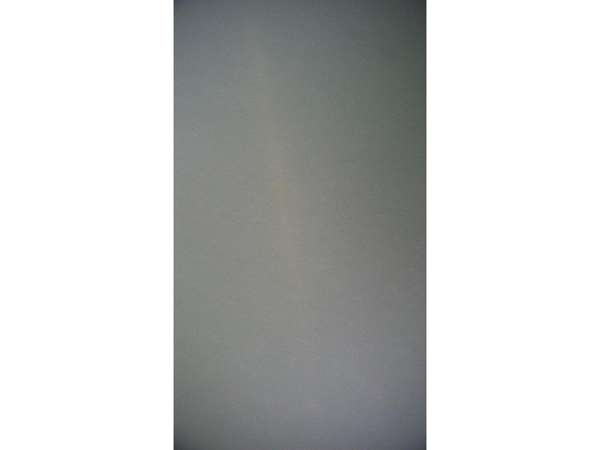
\includegraphics[height=0.3\textheight,width=0.5\textwidth]{imageProcessing/realPipe/001orgImstart.jpg}}&
\subfloat[Erkannte Objekte]{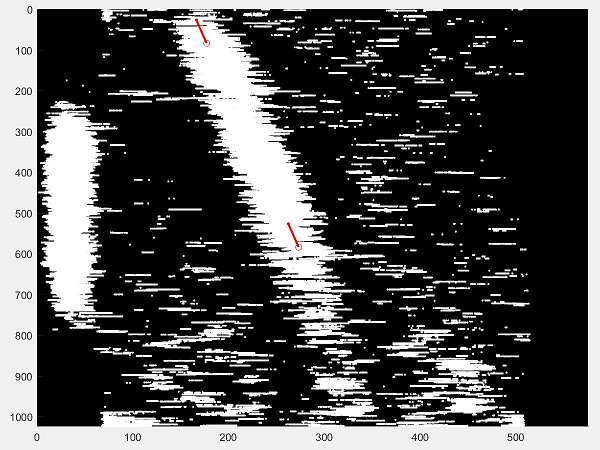
\includegraphics[height=0.3\textheight,width=0.5\textwidth]{imageProcessing/realPipe/001detectedImage.jpg}}
\end{tabular}
\caption[]{}
\end{figure}

\begin{figure}[H]
\begin{tabular}{cc}
\centering
\subfloat[Originalbild]{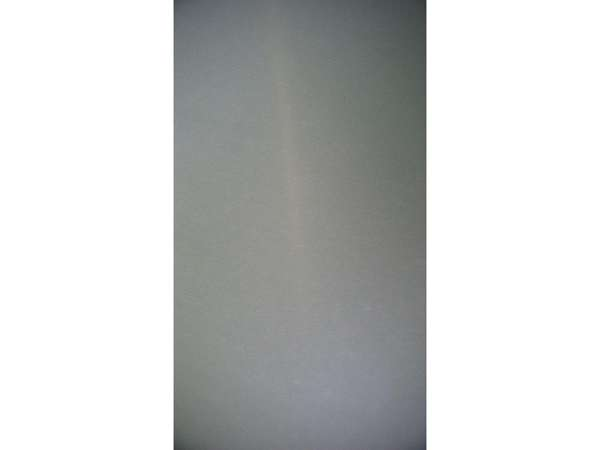
\includegraphics[height=0.3\textheight,width=0.5\textwidth]{imageProcessing/realPipe/002orgImstart.jpg}}&
\subfloat[Erkannte Objekte]{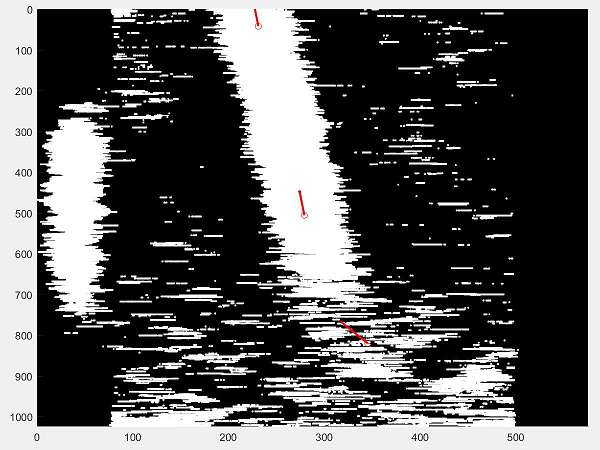
\includegraphics[height=0.3\textheight,width=0.5\textwidth]{imageProcessing/realPipe/002detectedImage.jpg}}
\end{tabular}
\caption[]{}
\end{figure}

\begin{figure}[H]
\begin{tabular}{cc}
\centering
\subfloat[Originalbild]{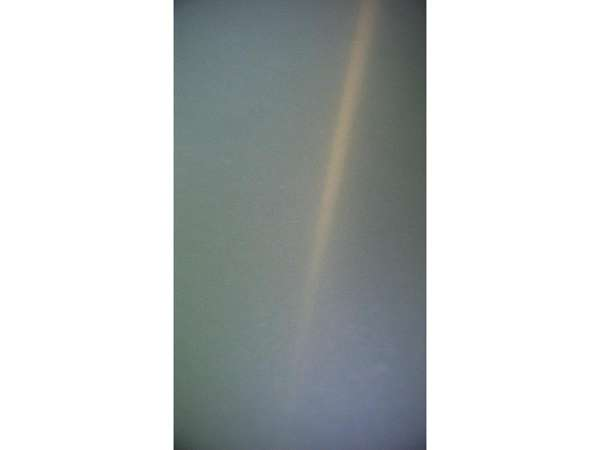
\includegraphics[height=0.3\textheight,width=0.5\textwidth]{imageProcessing/realPipe/003orgImstart.jpg}}&
\subfloat[Erkannte Objekte]{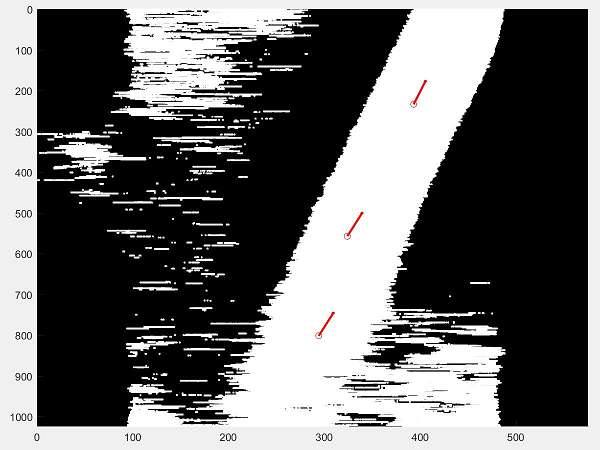
\includegraphics[height=0.3\textheight,width=0.5\textwidth]{imageProcessing/realPipe/003detectedImage.jpg}}
\end{tabular}
\caption[]{}
\end{figure}

\begin{figure}[H]
\begin{tabular}{cc}
\subfloat[Originalbild]{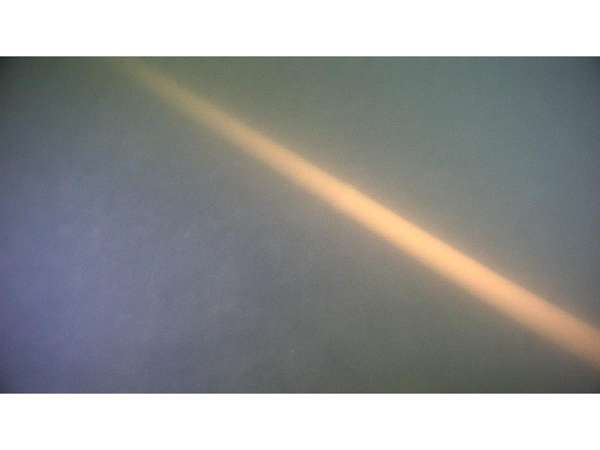
\includegraphics[height=0.3\textheight,width=0.5\textwidth]{imageProcessing/realPipe/004orgImstart.jpg}}&
\subfloat[Erkannte Objekte]{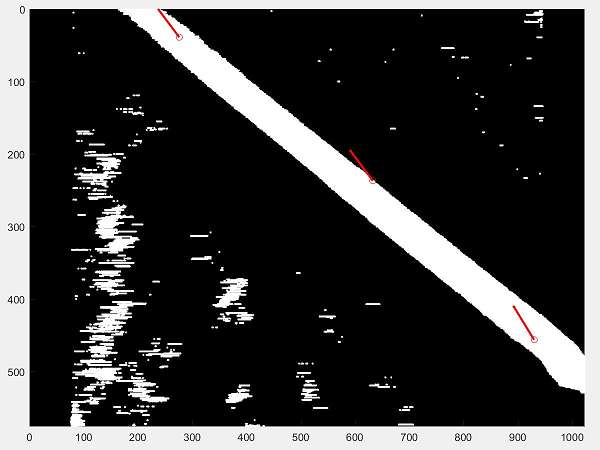
\includegraphics[height=0.3\textheight,width=0.5\textwidth]{imageProcessing/realPipe/004detectedImage.jpg}}
\end{tabular}
\caption[]{}
\end{figure}

\begin{figure}[H]
\begin{tabular}{cc}
\subfloat[Originalbild]{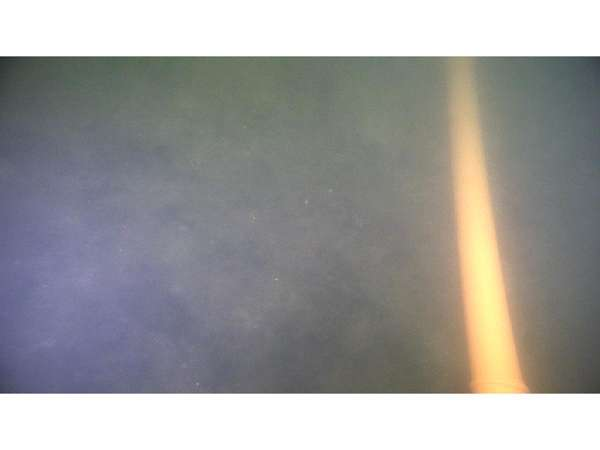
\includegraphics[height=0.3\textheight,width=0.5\textwidth]{imageProcessing/realPipe/005orgImstart.jpg}}&
\subfloat[Erkannte Objekte]{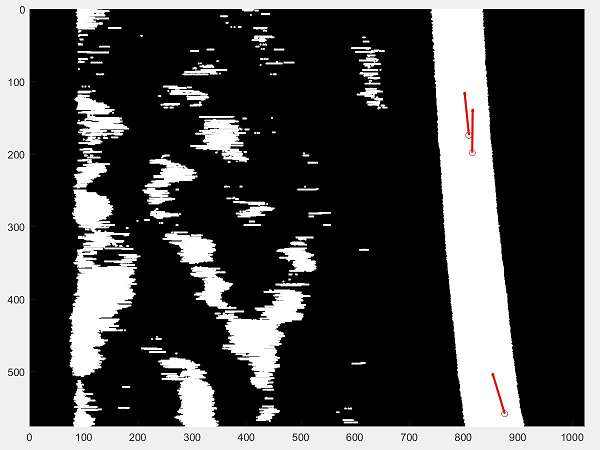
\includegraphics[height=0.3\textheight,width=0.5\textwidth]{imageProcessing/realPipe/005detectedImage.jpg}}
\end{tabular}
\caption[]{}
\end{figure}

\begin{figure}[H]
\begin{tabular}{cc}
\subfloat[Originalbild]{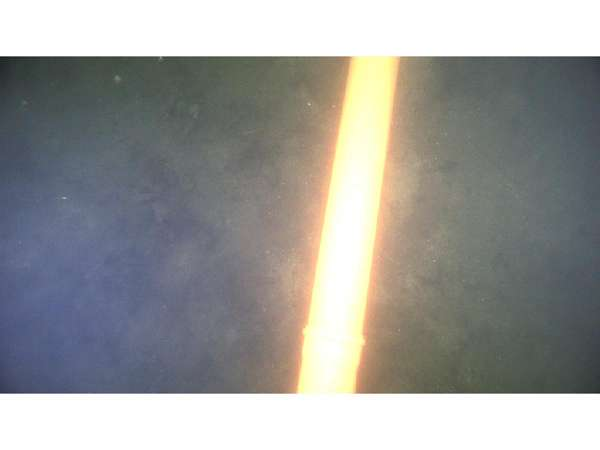
\includegraphics[height=0.3\textheight,width=0.5\textwidth]{imageProcessing/realPipe/006orgImstart.jpg}}&
\subfloat[Erkannte Objekte]{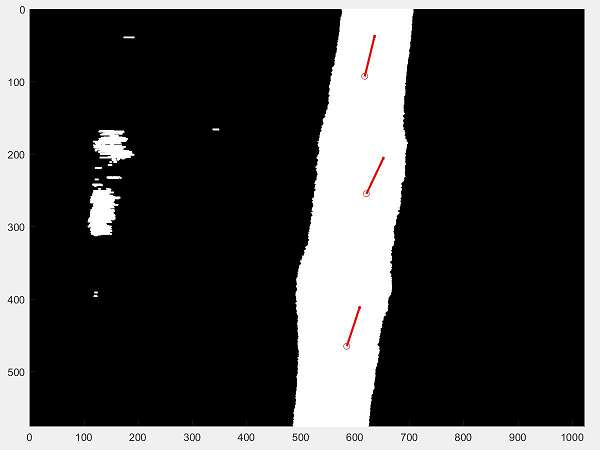
\includegraphics[height=0.3\textheight,width=0.5\textwidth]{imageProcessing/realPipe/006detectedImage.jpg}}
\end{tabular}
\caption[]{}
\end{figure}

\begin{figure}[H]
\begin{tabular}{cc}
\centering
\subfloat[Originalbild]{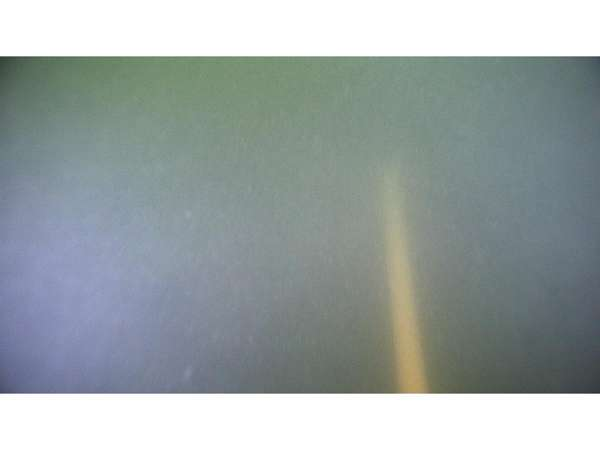
\includegraphics[height=0.3\textheight,width=0.5\textwidth]{imageProcessing/realPipe/007orgImstart.jpg}}&
\subfloat[Erkannte Objekte]{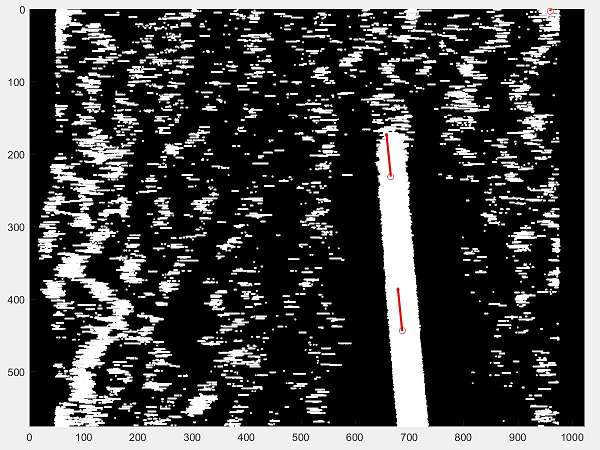
\includegraphics[height=0.3\textheight,width=0.5\textwidth]{imageProcessing/realPipe/007detectedImage.jpg}}
\end{tabular}
\caption[]{}
\end{figure}

\begin{figure}[H]
\begin{tabular}{cc}
\centering
\subfloat[Originalbild]{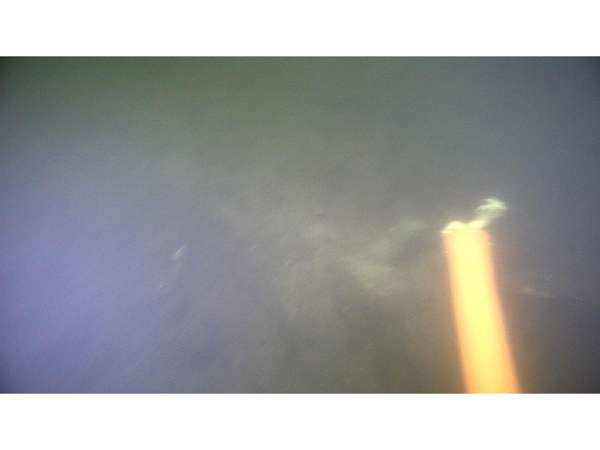
\includegraphics[height=0.3\textheight,width=0.5\textwidth]{imageProcessing/realPipe/008orgImstart.jpg}}&
\subfloat[Erkannte Objekte]{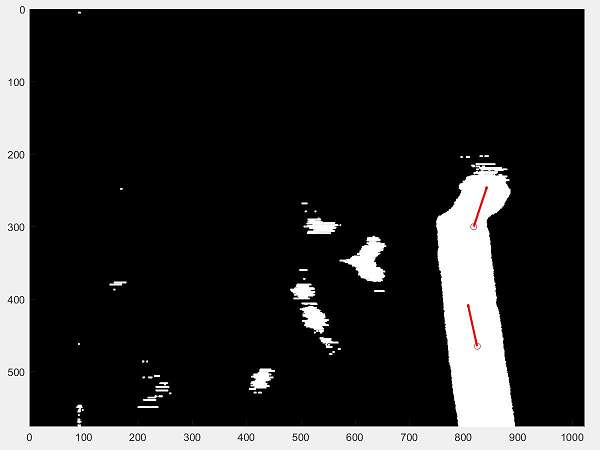
\includegraphics[height=0.3\textheight,width=0.5\textwidth]{imageProcessing/realPipe/008detectedImage.jpg}}
\end{tabular}
\caption[]{}
\end{figure}

\begin{figure}[H]
\begin{tabular}{cc}
\centering
\subfloat[Originalbild]{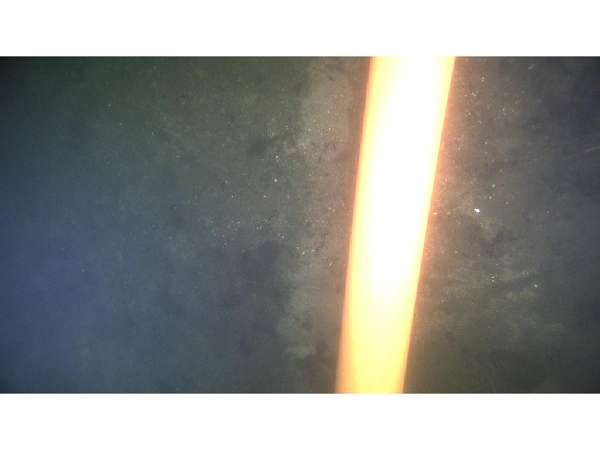
\includegraphics[height=0.3\textheight,width=0.5\textwidth]{imageProcessing/realPipe/009orgImstart.jpg}}&
\subfloat[Erkannte Objekte]{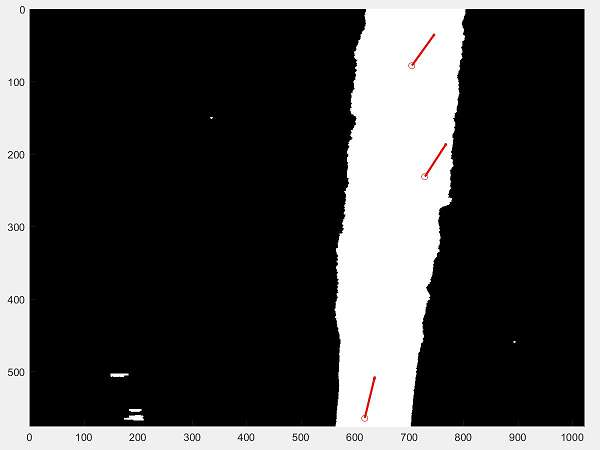
\includegraphics[height=0.3\textheight,width=0.5\textwidth]{imageProcessing/realPipe/009detectedImage.jpg}}
\end{tabular}
\end{figure}

\begin{figure}[H]
\begin{tabular}{cc}
\centering
\subfloat[Originalbild]{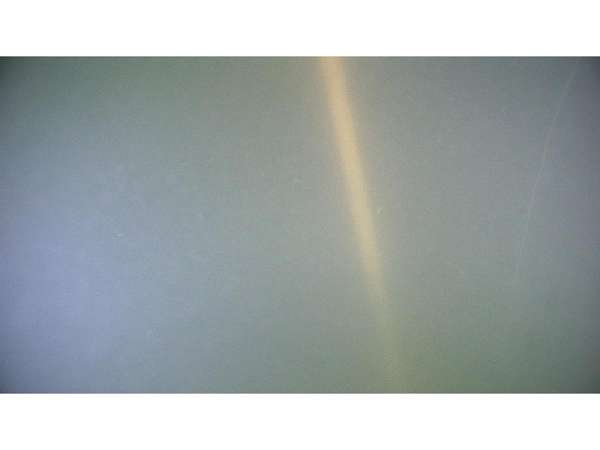
\includegraphics[height=0.3\textheight,width=0.5\textwidth]{imageProcessing/realPipe/010orgImstart.jpg}}&
\subfloat[Erkannte Objekte]{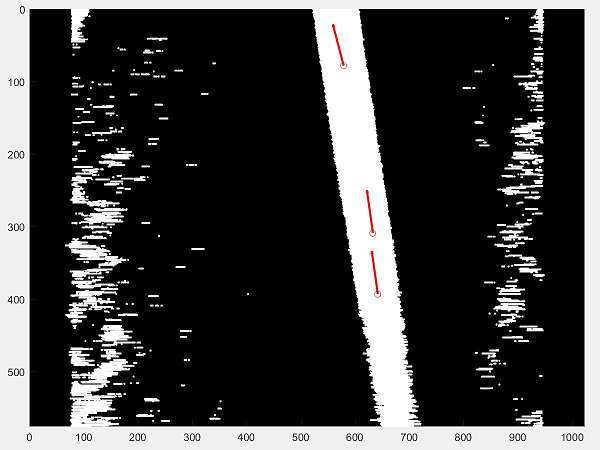
\includegraphics[height=0.3\textheight,width=0.5\textwidth]{imageProcessing/realPipe/010detectedImage.jpg}}
\end{tabular}
\caption[]{}
\end{figure}

\begin{figure}[H]
\begin{tabular}{cc}
\centering
\subfloat[Originalbild]{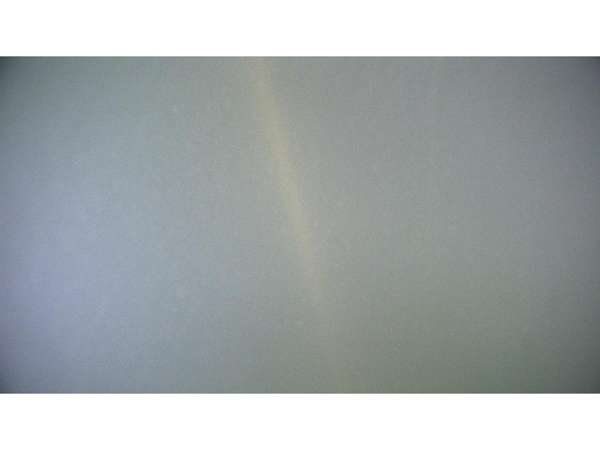
\includegraphics[height=0.3\textheight,width=0.5\textwidth]{imageProcessing/realPipe/011orgImstart.jpg}}&
\subfloat[Erkannte Objekte]{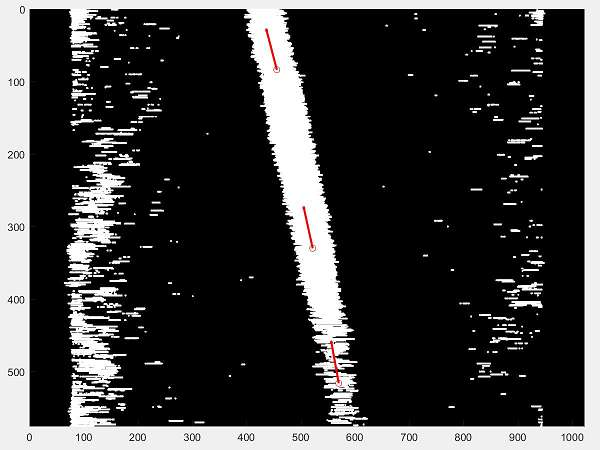
\includegraphics[height=0.3\textheight,width=0.5\textwidth]{imageProcessing/realPipe/011detectedImage.jpg}}
\end{tabular}
\caption[]{}
\end{figure}

\begin{figure}[H]
\begin{tabular}{cc}
\centering
\subfloat[Originalbild]{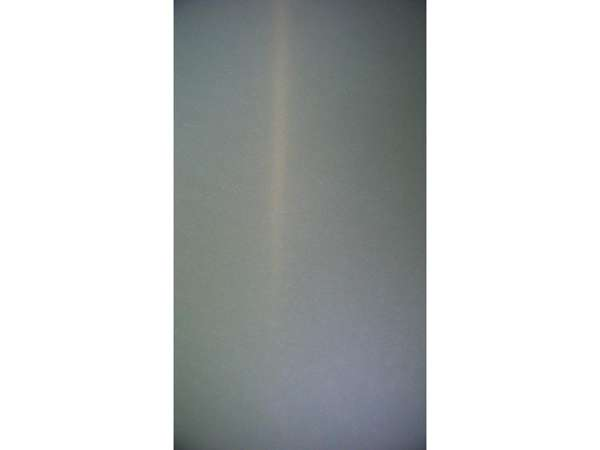
\includegraphics[height=0.3\textheight,width=0.5\textwidth]{imageProcessing/realPipe/012orgImstart.jpg}}&
\subfloat[Erkannte Objekte]{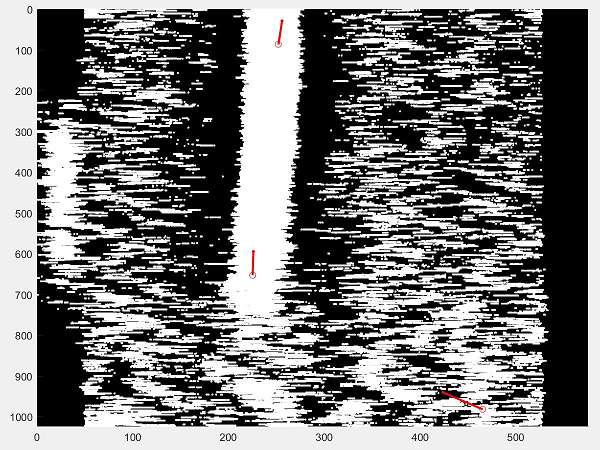
\includegraphics[height=0.3\textheight,width=0.5\textwidth]{imageProcessing/realPipe/012detectedImage.jpg}}
\end{tabular}
\caption[]{}
\end{figure}
